\apendice{Especificación de diseño}

\section{Introducción}
En este anexo se definirá la forma en que se han resuelto los requisitos expuestos anteriormente. Se dará una visión detallada de la arquitectura del sistema, diferenciando la aplicación web y el agente, o drone.

\section{Diseño de datos}
\subsection{WebApp}
La aplicación visible por el usuario final maneja los siguientes datos, o entidades:
\begin{itemize}
\item Usuario: Un usuario dispone de un nombre, apellidos, una dirección de correo electrónico, un nombre de usuario (que utilizará para iniciar sesión), y una contraseña cifrada. Se genera un id automáticamente para cada usuario.
\item Drone: Un drone dispone de un nombre, una localización, un controlador (que se corresponde con el id de usuario que lo controla), un puerto para el control remoto y un puerto para el feed de vídeo Se genera un id automáticamente para cada drone.
\item Registro de sesión: La aplicación web guarda registros del inicio/cierre de sesión por parte de un usuario. Dispone del identificador de usuario y de un timestamp.
\item Registro de intrusión: La aplicación web guarda registros de inicios de sesión infructuosos. Dispone del usuario utilizado, y un timestamp.
\item Registro de acciones: La aplicación web guarda registros de las acciones llevadas a cabo por cada usuario. Dispone de un identificador del usuario que realiza la acción, un timestamp y un identificador de la acción realizada.
\item Acciones: Se trata de las acciones que realizan los usuarios. Dispone de un identificador y una descripción de la acción.
\end{itemize}

\subsection{Agente}
El agente basa su funcionamiento en el uso de las siguientes entidades: 
\begin{itemize}
\item Controladores PID: Los controladores PID se encargan de proveer de valores para los diferentes canales automatizados del agente. Disponen de los coeficientes de las distintas componentes proporcional, integral y derivativa, así como de un límite superior y un límite inferior.
\item Sensores: Los sensores de distancia disponen de un pin de disparo, un pin de recepción del eco, y un ángulo.
\item Control Remoto: Se trata de un pequeño servidor encargado de recibir las órdenes de un usuario remoto. Dispone de una dirección y un puerto en el que escuchar. 
\item MSPio: Se trata de la implementación del protocolo MultiWiiSerialProtocol, el cual permite establecer comunicación con la controladora de vuelo. Dispone de un puerto serie y una velocidad de transferencia (en baudios).
\item Evasión de obstáculos: Se trata de la implementación del algoritmo VFH. Dispone de las siguientes entidades: 
	\begin{itemize}
	\item Malla de histograma: Una representación del entorno del agente. Dispone de las medidas de los sensores, distancias máxima y mínima a cubrir, el mapa del entorno, el tamaño de la ventana a cubrir, el tamaño de las celdas que componen la malla, una medida del error de los sensores y su apertura.
	\item Histograma polar: Una representación basada en sectores del entorno del agente. Dispone de una malla de histograma y el ancho de los sectores.
	\item Capa de salida: La capa de salida es la que realiza el cálculo de la orientación necesaria. Dispone de un histograma polar, un umbral de navegación segura, y la cantidad de sectores del histograma polar que se requieren para considerar un espacio como `amplio'.
	\end{itemize}
\item Sistema de localización: Se trata de la implementación del algoritmo del Filtro de Partículas. Dispone de una representación del entorno del agente, medidas de error para el control de rotación, de desplazamiento y de toma de medidas de los sensores, y el número de sectores a generar en cada celda. 
\end{itemize}


\begin{figure}[H]
	\centering
	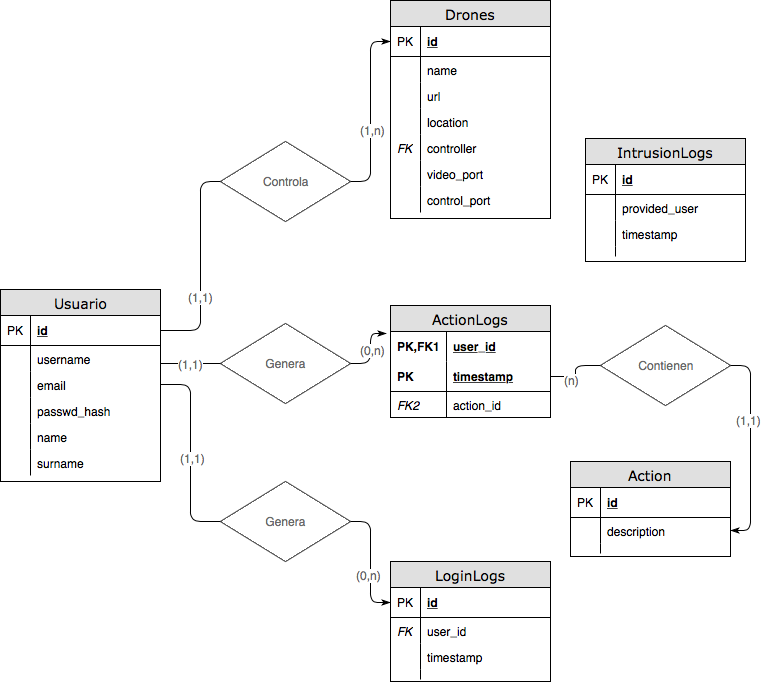
\includegraphics[width=0.9\textwidth]{ERFrontend}
	\caption{Diagrama E/R para WebApp.}\label{fig:erFront}
\end{figure}

\begin{figure}[H]
	\centering
	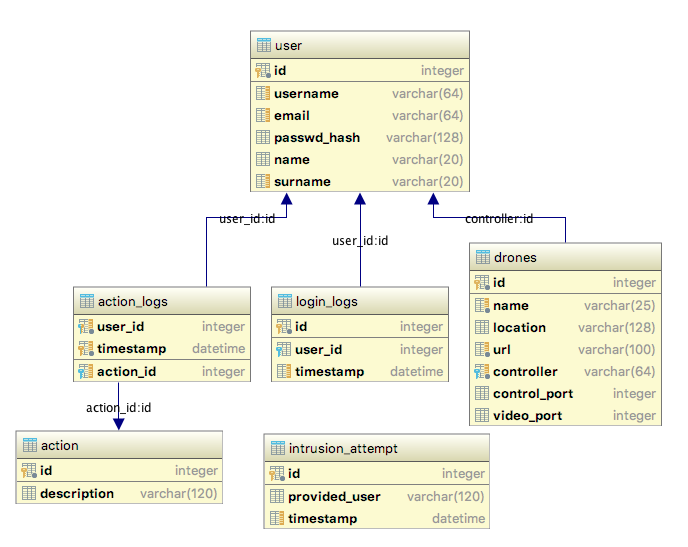
\includegraphics[width=0.9\textwidth]{erdiag}
	\caption[Diagrama Relacional WebApp]{Diagrama Relacional WebApp. Generado mediante PyCharm.}\label{fig:erdiag}
\end{figure}

\section{Diseño procedimental}
En este apartado se recoge el diagrama secuencial correspondiente a la totalidad  del sistema. En él, se representa el flujo de ejecución que puede o no, ver subsección \ref{subsec:patternCatalog}, seguir el sistema creado. 

\afterpage{
\begin{landscape}
\begin{figure}[H]
	\centering
	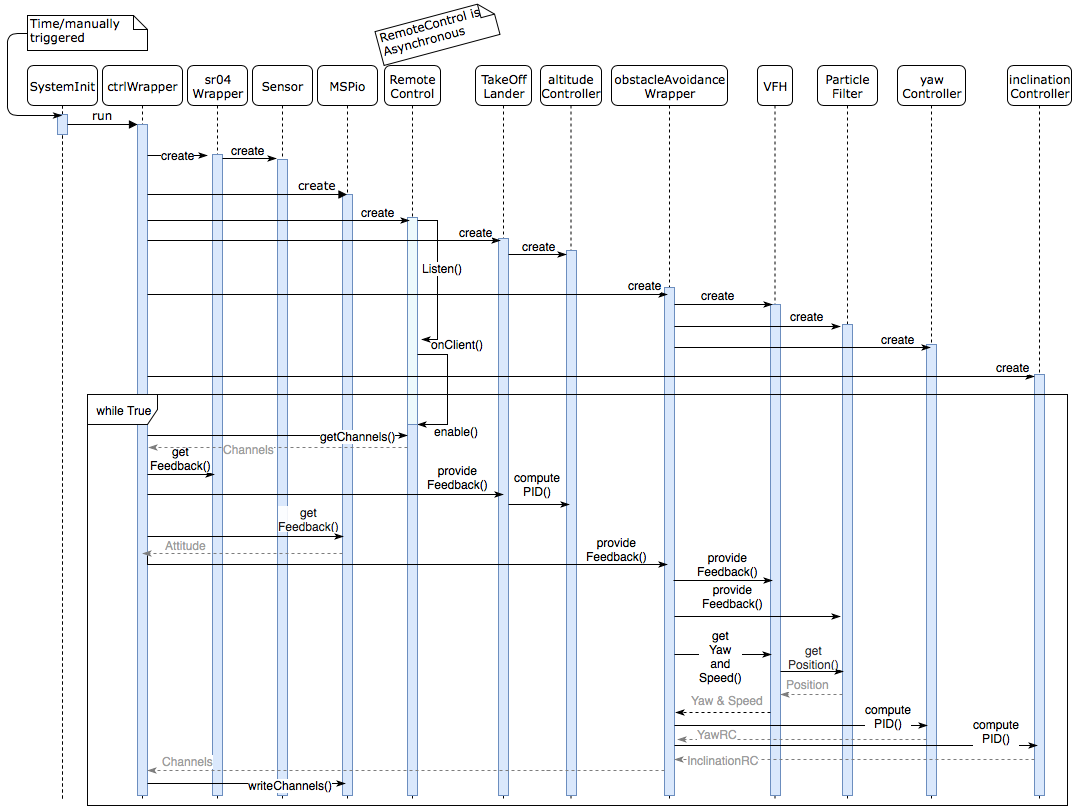
\includegraphics[width=1.2\textwidth]{SeqDiag}
	\caption[Diagrama de Secuencia]{Diagrama de secuencia del sistema.}\label{fig:SeqDiag}
\end{figure}
\end{landscape}
}



\section{Diseño arquitectónico}
En esta sección se dará una aclaración al diagrama \ref{fig:SeqDiag}, el cual da una idea general del funcionamiento del sistema. 
Para lograr un código fácil de mantener, y de escalar dado el potencial de crecimiento de las tecnologías relacionadas con este proyecto, se han generado una serie de clases intermedias que actúan a modo de \textit{wrapper}. La interfaz de la aplicación se ha generado siguiendo el conocido patrón MVC.

\subsection{Patrón MVC}
Para la parte representada por la aplicación web, se ha hecho uso del habitual patrón MVC (\textit{Model View Controller}), con la intención de separar la capa de lógica de la aplicación (\textit{Controller}), de la interfaz de usuario (\textit{View}) y de los datos manejados (\textit{Model}).

El patrón sigue la siguiente disposición: 
\begin{itemize}
\item \textbf{Model}: El modelo de la aplicación representa los datos a los que la aplicación accederá. Almacena los mismos y los gestiona. En el caso de este proyecto se trata de la base de datos de la aplicación Flask.
\item \textbf{View}: La vista de la aplicación muestra al usuario una interfaz gráfica sobre la que trabajar. Al recibir acciones, se encarga de solicitar al controlador las medidas necesarias. En el caso de este proyecto se corresponde con la interfaz web de la aplicación Flask.
\item \textbf{Controller}: El controlador podría considerarse el punto de comunicación entre el modelo y la vista. Se encarga de sincronizar los datos almacenados en el modelo con lo presentado en la vista, y de recibir los eventos generados por la vista y actuar en consecuencia.
\end{itemize}

\begin{figure}[H]
	\centering
	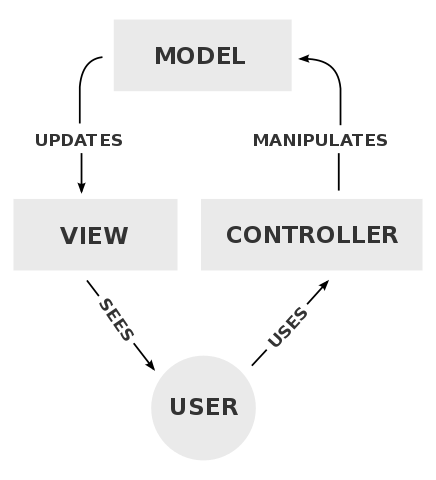
\includegraphics[width=0.5\textwidth]{mvc}
	\caption{Patrón MVC. Imagen de Wikipedia.}\label{fig:mvc}
\end{figure}

\subsection{Patrón Catálogo}
\label{subsec:patternCatalog}
El patrón catálogo no es tan habitual. Se utiliza sobre todo en lenguajes en los que se permite pasar una función o método como parámetro. Por ello en Python, donde todos los elementos son objetos de primera clase, es posible hacer uso de este patrón de forma muy sencilla. 

Permite establecer el comportamiento de una instancia más genérica, estableciendo los métodos generales de esta a métodos especializados de la clase que encapsula. En este caso, se encarga de proporcionar un acceso genérico a los métodos especializados de cada controlador automatizado. 

Este patrón es el núcleo de funcionamiento del sistema de control del agente. En el diagrama \ref{fig:SeqDiag} puede verse como se instancian numerosos controladores (\textit{RemoteControl, TakeOffLander} y  \textit{obstacleAvoidanceWrapper}). Dichos controladores, en el momento de ser instanciados por el \textit{ctrlWrapper} se encapsulan en una clase interna denominada \emph{PrioritizedController}. Dicha clase, podría ser considerada como la capa externa de un patrón proxy de protección\footnote{El patrón proxy de protección controla el acceso al objeto original}, el cual permite comprobar si el controlador está activo, si requiere de información de los sensores para su funcionamiento, y si requiere ser bloqueado para usarse (para protegerse de accesos simultáneos en el caso de tener un comportamiento asíncrono). Además, provee de información sobre la \emph{prioridad} del controlador. 

La prioridad de un controlador es lo que hace tan flexible el sistema. El diagrama \ref{fig:SeqDiag} presenta un uso secuencial de los diferentes \emph{PrioritizedController} generados, sin embargo, el orden de ejecución de cada uno, puede cambiar de forma dinámica. 
El \emph{ctrlWrapper} basa el procesamiento de los canales de control (Acelerador, Balanceo, Inclinación, Rotación, Armar/Desarmar... etc) en la prioridad de los controladores. 

Por ejemplo: Supongamos que existen dos controladores, uno remoto y manual (este es el usuario conectado al drone a través de la interfaz web) con una prioridad igual a $5$, y un controlador de rotación y velocidad autónomo, con una prioridad igual a $10$. 

La solicitud de los valores de los canales, se realiza por orden de prioridad de menor a mayor. De manera que el controlador automático de rotación y velocidad sobreescribirá el input del usuario (solo en los canales controlados), ya que tiene una prioridad superior. 
Supongamos que el usuario no desea eso. Prefiere ser él quien controle por completo el sistema, así que sencillamente arrancaría el sistema estableciéndose a si mismo como el controlador más prioritario. Sobreescribiendo de esta forma al controlador automatizado. 


\subsection{Arquitectura general}

La arquitectura de la parte visible del proyecto, la aplicación web, no presenta una complejidad elevada. Sin embargo el sistema de control del agente no es tan intuitivo. Por ello, se presenta el siguiente diagrama \ref{fig:arch} a modo aclaratorio.


\begin{figure}[H]
	\centering
	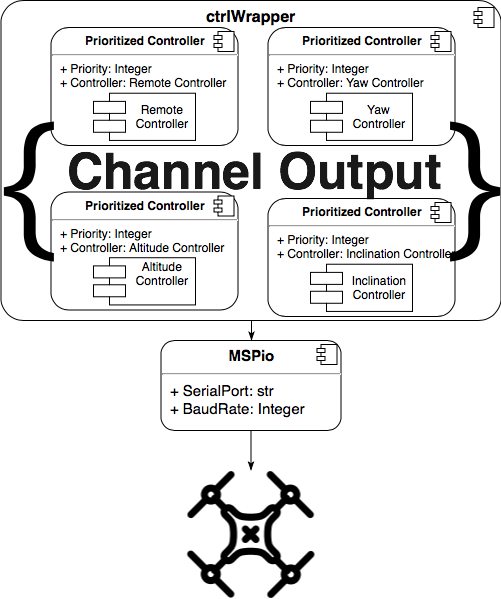
\includegraphics[width=0.9\textwidth]{arch}
	\caption[Arquitectura del sistema de control de agentes]{Encapsulación de controladores mediante controladores priorizados.}\label{fig:arch}
\end{figure}

El uso de esta arquitectura presenta varias ventajas: 
\begin{itemize}
\item Los controladores son independientes de la implementación del sistema de control. 
\item La arquitectura generada puede ser utilizada para controlar cualquier sistema basado en varios sistemas de control que se quieran priorizar. 
\item Permite llevar a cabo pruebas con mayor seguridad, dado que se puede hacer uso de un controlador manual solo cuando este se active, de manera que los controladores automatizados en pruebas puedan ser interrumpidos en cualquier momento. 
\end{itemize}


\subsection{Diseño de paquetes}

Para organizar las diferentes partes del proyecto, se ha generado una estructura de paquetes que diferencia la ubicación de los mismos (agente o servidor) de forma sencilla.

En la figura \ref{fig:backpackages} puede verse la estructura de paquetes seguida en el agente. Los paquetes contienen: 
\begin{itemize}
\item \textbf{algorithms}: Las implementaciones de los algoritmos empleados. 
\item \textbf{autoControllers}: Los diferentes sistemas de control automatizados implementados. 
\item \textbf{comms}: Los sistemas de comunicación implementados. Tanto entre el agente y la RaspberryPi, como entre el usuario y la RaspberryPi.
\item \textbf{sensors}: Las implementaciones de adquisición de datos de los sensores usados.
\item \textbf{systemControl}: Contiene la implementación del sistema de control del agente.
\end{itemize}

\begin{figure}[H]
	\centering
	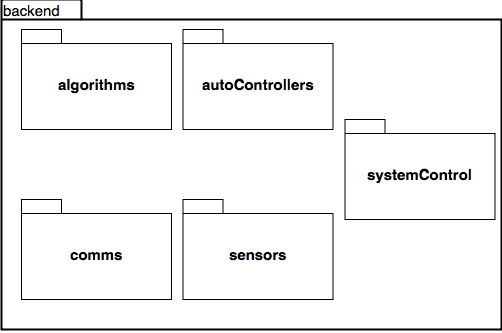
\includegraphics[width=0.9\textwidth]{backendpackages}
	\caption[Estructura de paquetes en agente]{Estructura de los paquetes en el agente.}\label{fig:backpackages}
\end{figure}

En la figura \ref{fig:frontpackages} puede verse la estructura de paquetes seguida en el servidor web. Los paquetes contienen: 
\begin{itemize}
\item \textbf{controller}: Contiene la implementación del controlador de la aplicación web.
\item \textbf{model}: Contiene la implementación del modelo de datos utilizado por el controlador.
\begin{itemize}
\item \textit{migrations}: Contiene un mecanismo para realizar operaciones de upgrade/downgrade de las diferentes versiones de la base de datos.
\begin{itemize}
\item versions: Contiene las versiones de la base de datos
\end{itemize}
\end{itemize}
\item \textbf{view}: Contiene la vista de la aplicación web.
\begin{itemize}
\item \textit{static}: Contiene los elementos estáticos de la aplicación web.
\item \textit{templates}: Contiene las plantillas que representan la interfaz de la aplicación web.
\end{itemize}
\end{itemize}

\begin{figure}[H]
	\centering
	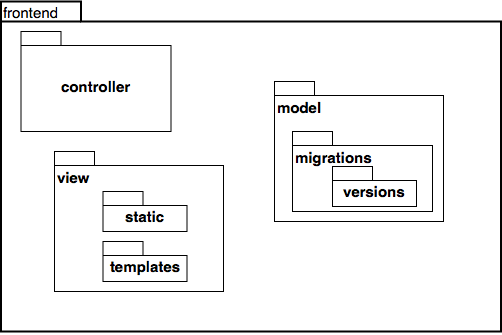
\includegraphics[width=0.9\textwidth]{frontendpackages}
	\caption[Estructura de paquetes en servidor web]{Estructura de los paquetes en el servidor web.}\label{fig:frontpackages}
\end{figure}

\subsection{Diseño de clases}

Siguiendo con la nomenclatura utilizada en el diseño de la estructura de paquetes, se dará a continuación las características de cada clase implementada: 
\subsubsection{FrontEnd}
\begin{itemize}
\item \texttt{\textbf{controller}.\_\_init\_\_}: Establece una serie de opciones necesarias para el arranque de la aplicación web. Rutas de archivos, instancia la aplicación en sí, establece la configuración, la base de datos, el servicio de login y la capa de sockets utilizada para comunicar la interfaz de usuario de forma asíncrona con la aplicación.
\item \texttt{\textbf{controller}.routes}: Se trata de la clase encargada del control de la aplicación web. Responde a las solicitudes de los usuarios realizando las acciones correspondientes, y establece la comunicación necesaria entre el agente y el usuario.
\item \texttt{\textbf{model}.config}: Se trata de una clase que contiene elementos de configuración de la aplicación web. Tal como la ubicación de la base de datos a utilizar, la clave secreta para generar los tokens de la aplicación, etc.
\item \texttt{\textbf{model}.models}: Se trata de la definición de las entidades a utilizar por el ORM utilizado (SQLAlchemy).
\item \texttt{\textbf{model}.migrations.env}: Se trata de un script generado por Alembic (una extensión para SQLAlchemy que permite realizar versionado de las bases de datos), y que permite actualizar, o revertir, los cambios realizados basándose en las diferentes versiones generadas. 
\item \texttt{\textbf{model}.migrations.versions.XXXXXX}: Se trata de los diferentes scripts que usará Alembic para actualizar o revertir los cambios realizados en la base de datos.
\item \texttt{\textbf{view}.login}: Un formulario simple a utilizar por el controlador a la hora de obtener los datos de login.
\item \texttt{\textbf{frontend}.droneControlWebUI}: El instanciador del servidor web. Se encarga de ejecutar la aplicación web mediante los parámetros especificados.
\end{itemize}


\begin{figure}[H]
	\centering
	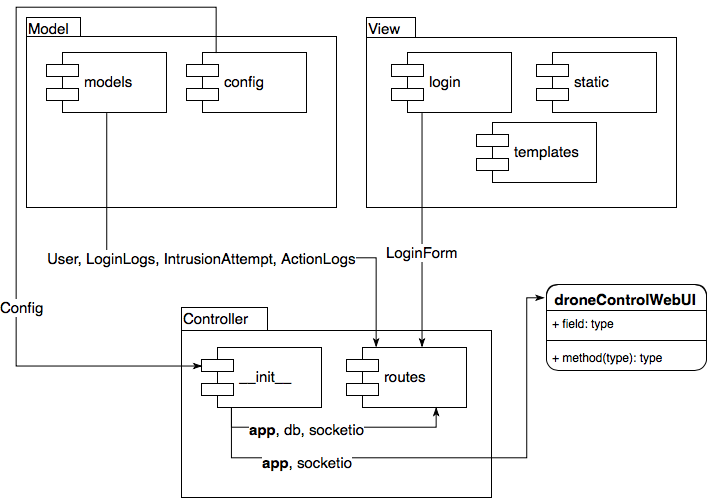
\includegraphics[width=0.9\textwidth]{frontendClassDiag}
	\caption[Diagrama de clases FrontEnd]{Diagrama de clases del frontend.}\label{fig:frontendClassDiag}
\end{figure}



\subsubsection{BackEnd}

\begin{itemize}
\item \texttt{\textbf{algorithms}.Geometry}: Se trata de un módulo auxiliar utilizado por el Filtro de Partículas para realizar cálculos geométricos de forma vectorizada haciendo uso de Numpy.
\item \texttt{\textbf{algorithms}.ParticleFilter}: Se trata de la implementación del Filtro de Partículas. Se encarga de obtener la posición del agente en el plano.
\item \texttt{\textbf{algorithms}.VFH}: Se trata de la implementación del sistema de evasión de obstáculos. 
\item \texttt{\textbf{autoControllers}.abcControllerPID}: Se trata de una metaclase\footnote{En Python las interfaces se denominan \emph{metaclases}, aunque las capacidades de estas son más extendidas, servirá para referirnos a ellas de aquí en adelante.} que define el contrato que deben subscribir las clases que implementen controladores PID.
\item \texttt{\textbf{autoControllers}.altitudeController}: Se trata de una implementación de la metaclase abcControllerPID, destinada al control de altitud.
\item \texttt{\textbf{autoControllers}.inclinationController}: Se trata de una implementación de la metaclase abcControllerPID, destinada al control de inclinación.
\item \texttt{\textbf{autoControllers}.yawController}: Se trata de una implementación de la metaclase abcControllerPID, destinada al control de la orientación.
\item \texttt{\textbf{autoControllers}.obsAvoidanceWrapper}: Se trata de una clase implementada para encapsular los algoritmos de evasión de obstáculos, y generar el cálculo del control de orientación e inclinación para alimentar los controladores PID correspondientes.
\item \texttt{\textbf{autoControllers}.takeOffLanding}: Se trata de una clase implementada para encapsular el controlador de altitud. Permite tanto el despegue como el aterrizaje, y genera el cálculo del control de altitud para alimentar al controlador PID correspondiente. 
\item \texttt{\textbf{comms}.MultiWiiProtocol}: Esta es la implementación del protocolo MultiWiiSerial Protocol. Dicho protocolo es utilizado por las herramientas de configuración de las controladoras de vuelo de los \emph{drones} actuales, que ejecutan un firmware basado en el controlador MultiWii. Se encarga de llevar a cabo la comunicación entre el drone y la RaspberryPi, permitiendo el flujo de información en ambas direcciones. 
\item \texttt{\textbf{comms}.RemoteControl}: Se trata del servidor encargado de recibir las órdenes remotas del usuario.
\item \texttt{\textbf{sensors}.sr04Wrapper}: Se trata de una pequeña clase que encapsula el acceso a los sensores de ultrasonidos utilizados para el cálculo de distancias, para el sistema de evasión de obstáculos.
\item \texttt{\textbf{sensors}.Sensor}: Se trata de una pequeña clase que representa un sensor de ultrasonidos, incluyendo el acceso a la instancia de la clase \emph{Echo} (perteneciente a la librería \emph{Bluetin\_Echo} ), así como el ángulo en el que está orientado el sensor, y los pines a los que está conectado.
\item \texttt{\textbf{systemControl}.ctrlWrapper}: Se trata de la implementación del sistema de control del drone. Se posiciona como un mecanismo de separación entre el drone y sus sensores, y los diferentes controladores. Se encarga de coordinar, de forma priorizada, los diferentes mecanismos de control del agente, así como de suministrar a aquellos que así lo requieran la información de los diferentes sensores a los que tiene acceso.
\end{itemize}

Se dispone de un diagrama de clases del backend en la figura \ref{fig:backendClassDiag}. Se han añadido colores para tratar de aumentar la claridad del diagrama, de por sí algo complejo.
\newpage



\begin{figure}[H]
	\centering
	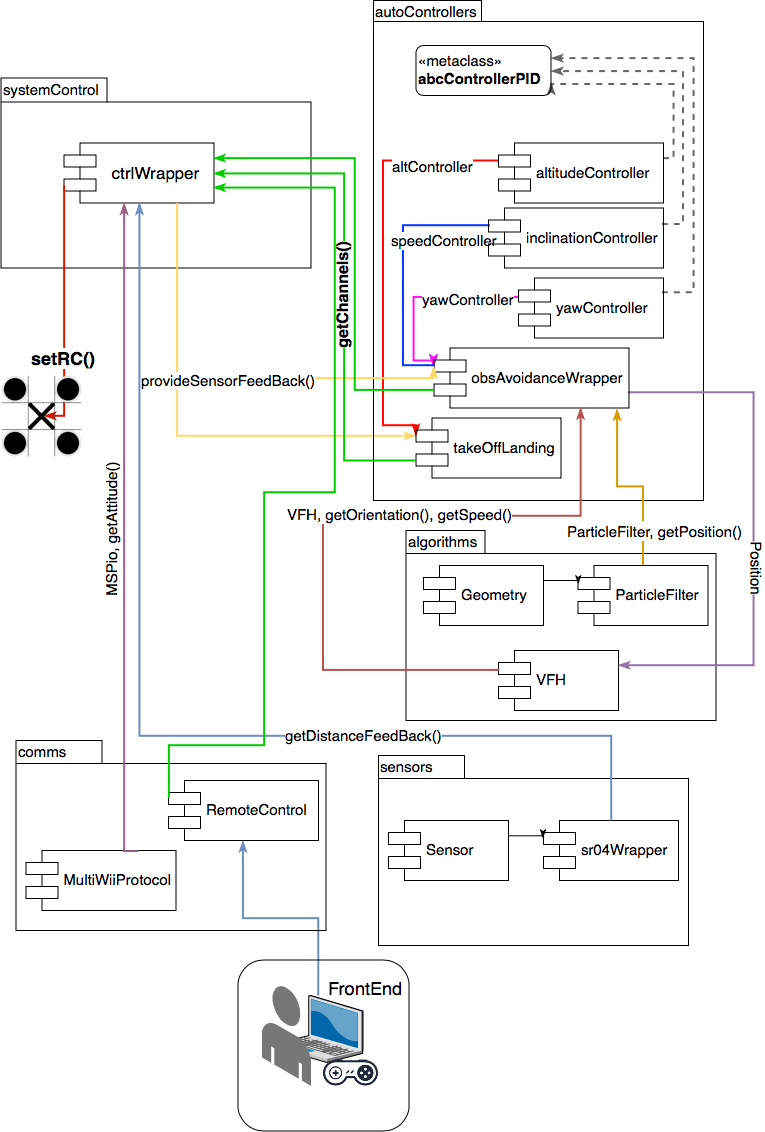
\includegraphics[width=1\textwidth]{backendClassDiag}
	\caption[Diagrama de clases BackEnd]{Diagrama de clases del backend.}\label{fig:backendClassDiag}
\end{figure}





















